\section{Performance Evaluation}
\label{sec:Performance}

We conducted our \teledroid\ application in three different mode: scan mode, monitor mode, and lazy mode. In scan mode, local device and server will output their own list of files along with their modified time. Then, \teledroid\ compares the two lists with the modified time to determine whether the file should be sync from one side to the other. In monitor mode, we enable inotify process on both server side and client side to monitor the changed file. Once the file is changed, inotify will report to \teledroid\ and request to sync that file. In lazy mode, even when the file has been changed on either side, that file will not be synced until it is read by \teledroid. In a limit of time, we can not complete the functionality for lazy mode. Thus, lazy mode will be our future work and was not be used in our experiment.
In our experiments, ......

\subsection{Testing Plan}
(Riku)
Plan:\\
	- scan mode\\
	- monitor mode\\
	- lazy mode (Future work)\\
	
	sample:	
		- one Large-size file\\
		- multiple small-size files\\
		(with new or modified files)\\
				
\subsection{Hardware Configuration}
Our test device is an Android Dev Phone 1. There are one Qualcomm 7210 processor in 528MHZ and 192 MB RAM memory in Android 
Dev Phone 1. With a touch screen and a trackball for navigation, it also provides QWERTY slider keyboard for input. Wi-Fi, 
GPS,  and Bluetooth v2.0 are all supported in Android Dev Phone 1. For network standard of cellular provider, it can 
support 3G WCDMA in 1700/2100 MHz and Quad-band GSM in 850/900/1800/1900 MHz. Note that Android Dev Phone 1 includes 1GB 
MicroSC card as an external hard drive. It can be replaced with up to 16GB card. Concerning network environment, we 
proposed to connect to CSLabs network in University of San Francisco using Wi-Fi connection.

\subsection{Results}
The results of CPU usage is shown in Figure~\ref{fig:cpu}. However it is not as we expected. The monitor mode didn't gain 
significant advantage over scan mode. However, they synchronization finished faster than scan mode. So the overall cpu 
usage should be lower than the run-time cpu usage. 

\begin{figure}%[htp]
\centering
\subfigure[CPU Usage in Monitor Mode]{\label{fig:cpu-monitor}
    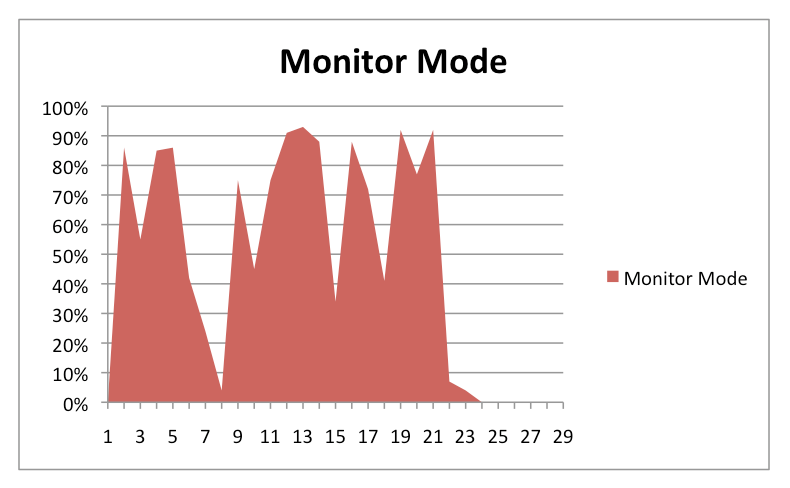
\includegraphics[scale=0.5]{cpu_monitor}}
\hspace{0.20in}
\subfigure[CPU Usage in Scan Mode]{\label{fig:cpu-scan}
	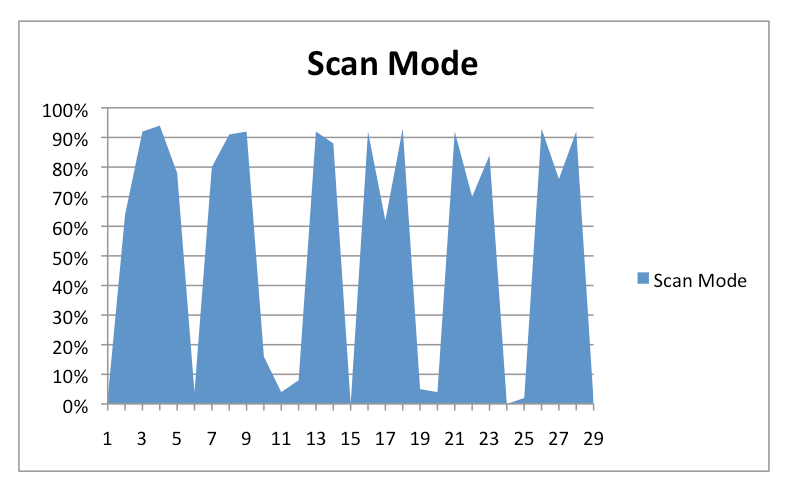
\includegraphics[scale=0.5]{cpu_scan}}
\subfigure[Comparison of CPU Usage]{\label{fig:cpu-comp}
    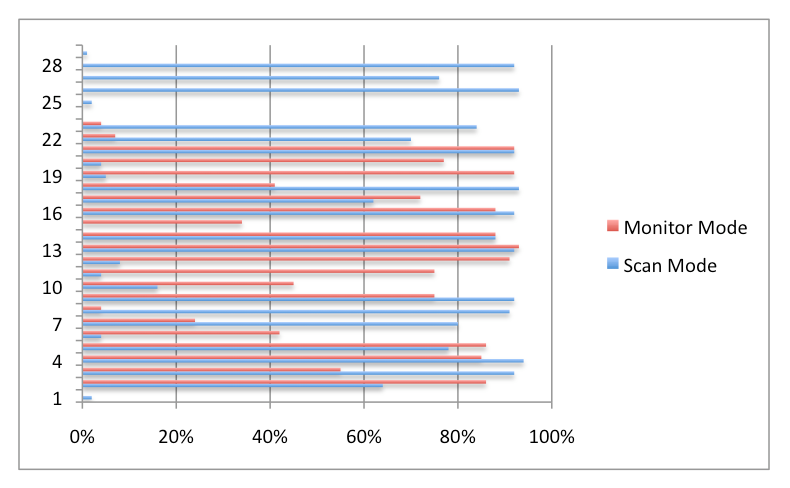
\includegraphics[scale=0.7]{cpu}}
\caption{The CPU usage comparison of Monitor and Scan mode}
\label{fig:cpu}
\end{figure}

The same as CPU usage, the memory usage data is also disappointed. As shown in Figure~\ref{fig:memory}, the memory usage in 
monitor mode is even higher than scan mode. We think this is due to our implementation use only \verb+ScanFileThread+ in 
scan mode while using an extra \verb+FileMonitorThread+ in monitor thread. 

\begin{figure}%[htp]
\centering
\subfigure[Memory Usage in Monitor Mode]{\label{fig:memory-monitor}
    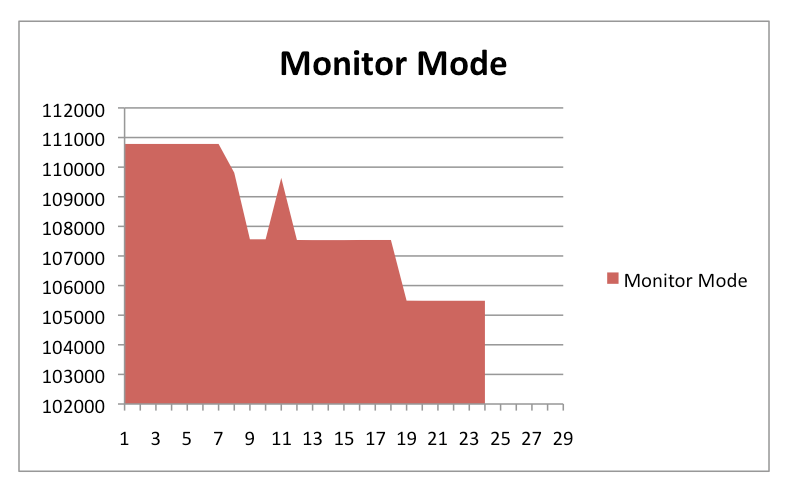
\includegraphics[scale=0.5]{memory_monitor}}
\hspace{0.20in}
\subfigure[Memory Usage in Scan Mode]{\label{fig:memory-scan}
	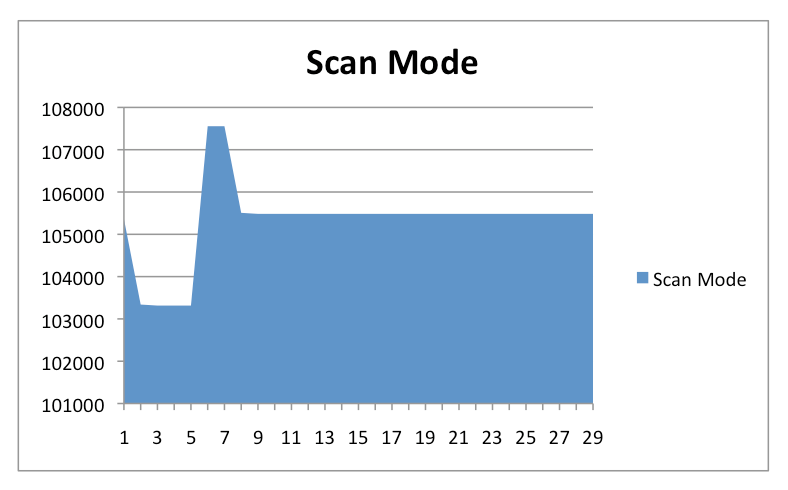
\includegraphics[scale=0.5]{memory_scan}}
\subfigure[Comparison of Memory Usage]{\label{fig:memory-comp}
    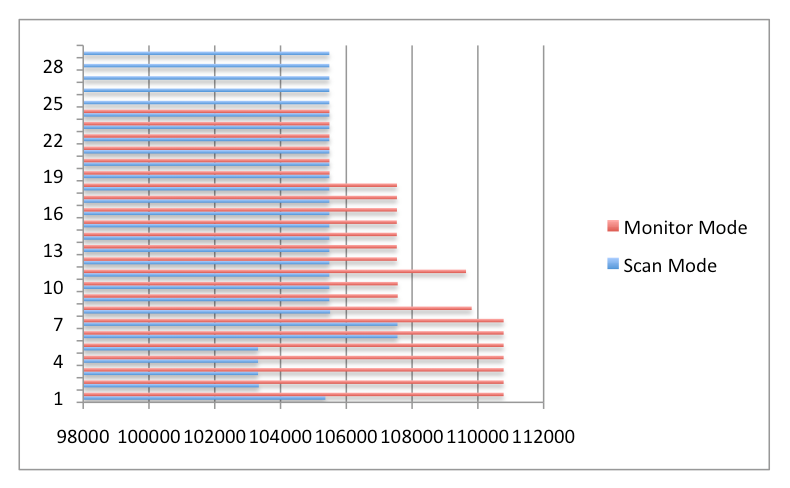
\includegraphics[scale=0.7]{memory}}
\caption{The Memory usage comparison of Monitor and Scan mode}
\label{fig:memory}
\end{figure}

In the test of synchronization speed, we finally got the data represent the the performance of monitor version is better. 
As we can see in Figure~\ref{fig:speed}, the speed of monitor mode is faster than scan mode on client side. However, the 
server didn't show significant differences. This may be due to our current server side script using a pull-sync instead of push-sync as client side. 
\begin{figure}[htp]
\centering
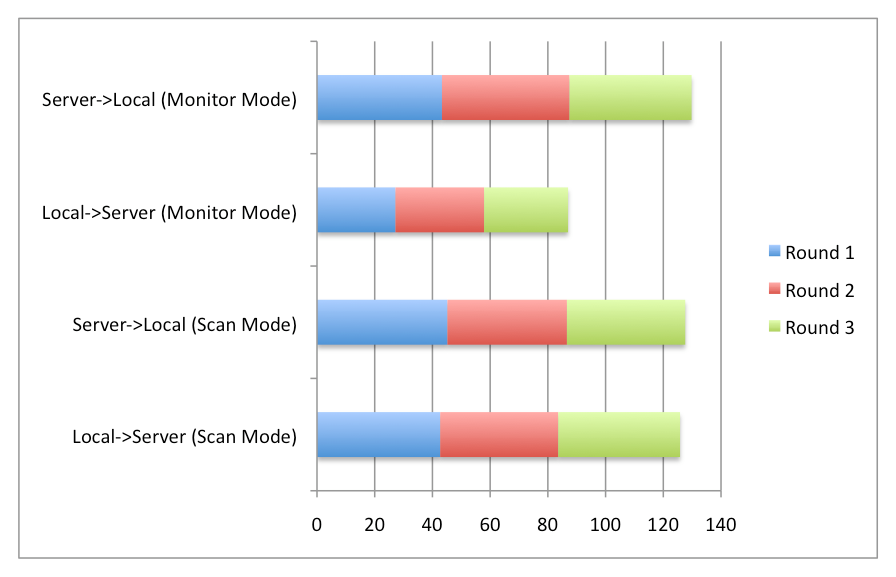
\includegraphics[scale=0.7]{speed}
\caption{Comparison of Synchronization Speed}\label{fig:speed}
\end{figure}
